\documentclass[a4paper,10pt]{article}
\usepackage[utf8]{inputenc}
\usepackage[a4paper,
            bindingoffset=0.2in,
            left=1in,
            right=1in,
            top=1in,
            bottom=1in,
            footskip=.25in]{geometry}

%###############################################################################

%\input{~/layout/global_layout}


%###############################################################################

% packages begin

\usepackage[
  backend=biber,
  sortcites=true,
  style=alphabetic,
  eprint=true,
  backref=true
]{biblatex}
\addbibresource{bibliographie.bib}
\usepackage[acronym]{glossaries}
\usepackage{euscript}[mathcal]
% e.g. \mathcal{A} for fancy letters in mathmode
\usepackage{amsmath,amssymb,amstext,amsthm}

\usepackage{mdframed}
\newmdtheoremenv[nobreak=true]{problem}{Problem}[subsection]
\newmdtheoremenv[nobreak=true]{claim}{Claim}[subsection]
\newtheorem{definition}{Definition}[subsection]
\newtheorem{lemma}{Lemma}[claim]
\newtheorem{plemma}{Lemma}[problem]

\usepackage{mathtools}
\DeclarePairedDelimiter\ceil{\lceil}{\rceil}
\DeclarePairedDelimiter\floor{\lfloor}{\rfloor}

\usepackage{enumerate}
\usepackage[pdftex]{graphicx}
\usepackage{subcaption}
% 'draft' für schnelleres rendern mitübergeben -> [pdftex, draft]
% dadruch wird nicht das bild mitgerendered, sondern nur ein kasten mit bildname -> schont ressourcen

\usepackage{hyperref}

\usepackage{tikz}
\usetikzlibrary{arrows,automata,matrix,positioning,shapes}

% for adding non-formatted text to include source-code
\usepackage{listings}
\lstset{language=Python,basicstyle=\footnotesize}
% z.B.:
% \lstinputlisting{source_filename.py}
% \lstinputlisting[lanugage=Python, firstline=37, lastline=45]{source_filename.py}
%
% oder
%
% \begin{lstlisting}[frame=single]
% CODE HERE
%\end{lstlisting}
\usepackage{algorithm}
\usepackage{algpseudocode}

\usepackage{wasysym}

\usepackage{titling}
\usepackage{titlesec}
\usepackage[nocheck]{fancyhdr}
\usepackage{lastpage}

\usepackage{kantlipsum}
\usepackage[colorinlistoftodos,prependcaption,textsize=tiny]{todonotes}

\usepackage{svg}

% packages end
%###############################################################################

\pretitle{% add some rules
  \begin{center}
    \LARGE\bfseries
} %, make the fonts bigger, make the title (only) bold
\posttitle{%
  \end{center}%
  %\vskip .75em plus .25em minus .25em% increase the vertical spacing a bit, make this particular glue stretchier
}
\predate{%
  \begin{center}
    \normalsize
}
\postdate{%
  \end{center}%
}

\titleformat*{\section}{\Large\bfseries}
\titleformat*{\subsection}{\large\bfseries}
\titleformat*{\subsubsection}{\normalsize\bfseries}

\titleformat*{\paragraph}{\Large\bfseries}
\titleformat*{\subparagraph}{\large\bfseries}

%###############################################################################

\pagestyle{fancy}
\fancyhf{}
% l=left, c=center, r=right; e=even_pagenumber, o=odd_pagenumber; h=header, f=footer
% example: [lh] -> left header, [lof,ref] -> fotter left when odd, right when even
%\fancyhf[lh]{}
%\fancyhf[ch]{}
%\fancyhf[rh]{}
%\fancyhf[lf]{}
\fancyhf[cf]{\footnotesize Page \thepage\ of \pageref*{LastPage}}
%\fancyhf[rf]{}
\renewcommand{\headrule}{} % removes horizontal header line

% Fotter options for first page

\fancypagestyle{firstpagestyle}{
  \renewcommand{\thedate}{\textmd{}} % removes horizontal header line
  \fancyhf{}
  \fancyhf[lh]{\ttfamily M.Sc. Computer Science\\KTH Royal Institute of Technology}
  \fancyhf[rh]{\ttfamily Period 4\\\today}
  \fancyfoot[C]{\footnotesize Page \thepage\ of \pageref*{LastPage}}
  \renewcommand{\headrule}{} % removes horizontal header line
}
%###############################################################################

\newcommand\extrafootertext[1]{%
    \bgroup
    \renewcommand\thefootnote{\fnsymbol{footnote}}%
    \renewcommand\thempfootnote{\fnsymbol{mpfootnote}}%
    \footnotetext[0]{#1}%
    \egroup
}

%###############################################################################

\title{
  \normalsize{DD2356 VT25 Methods in}\\
  \normalsize{High Performance Computing}\\
  \large{Assignment 3}
}
\author{
  \small Rishi Vijayvargiya\textsuperscript{\textdagger}\\[-0.75ex]
%  \footnotesize\texttt{MN: }\\[-1ex]
  \scriptsize\texttt{rishiv@kth.se}
  \and
  \small Paul Mayer\textsuperscript{\textdagger}\\[-0.75ex]
%  \footnotesize\texttt{MN: }\\[-1ex]
  \scriptsize\texttt{pmayer@kth.se}
  \and
  \small Lennart Herud \textsuperscript{\textdagger}\\[-0.75ex]
%  \footnotesize\texttt{MN: }\\[-1ex]
  \scriptsize\texttt{herud@kth.se}
}
\date{}

%###############################################################################
% define Commands

\newcommand{\N}{\mathbb{N}}
\newcommand{\R}{\mathbb{R}}
\newcommand{\Z}{\mathbb{Z}}
\newcommand{\I}{\mathbb{I}}

\newcommand{\E}{\mathbb{E}}
\newcommand{\Prob}{\mathbb{P}}

\renewcommand{\epsilon}{\varepsilon}

%###############################################################################
\makeatletter
\renewcommand*{\@fnsymbol}[1]{\ensuremath{\ifcase#1\or \dagger\or \ddagger\or
   \mathsection\or \mathparagraph\or \|\or **\or \dagger\dagger
   \or \ddagger\ddagger \else\@ctrerr\fi}}
\makeatother
%###############################################################################

\begin{document}
\maketitle
\extrafootertext{\textsuperscript{\textdagger}Authors made equal contribution to the project}
\thispagestyle{firstpagestyle}

\listoftodos
\vspace{1em}

% content begin
%

\section*{Prefix}
The code for our project can be found at this location: \url{https://github.com/paulmyr/DD2356-MethodsHPC/tree/master/3_open_mp}. 

\tableofcontents
\newpage

\todo[inline]{Check headers}

\section{Exercise 1 - OpenMP Hello World}
\subsection{Question 1 - Write an OpenMP C code with each thread printing Hello World from Thread X! where X is the thread ID.}
We wrote the c code using the lecture material. The code is attachted in the GitHub repository.
The output looks as follows (exercise1/output.txt):
Hello World from Thread 0! \\
Hello World from Thread 2! \\
Hello World from Thread 1! \\
Hello World from Thread 3! \\


\subsection{Question 2 - How do you compile the code? Which compiler and flags have you used?}
We compile the code using \verb|gcc| compiler. 
The code is compiled using the \verb|-fopenmp| flag to utilize \verb|OpenMP|. The full command is: 
$ srun -n 1 gcc -fopenmp a3/ex1/hello_world.c -o a3/ex1/hello_world.out$
We attached the slurmfile to run the code on \verb|Dardel| in the repo (\verb|ex1.slurm|).

\subsection{Question 3 - Use what you've learned from hwloc/numactl to discover how many cores your job is allocated with. }
The hwloc output can be found \href{https://github.com/paulmyr/DD2356-MethodsHPC/blob/master/3_open_mp/img/ex1/topology.svg}{here}.
We can observe that four virtual cores are being utilized on two physical cores. We can see the 4 specified (virtual) CPU cores from our 
jobscript in the figure.

\subsection{Question 4 - How do you run the OpenMP code on Dardel? What flags did you set?}
As stated in question 2, we use the \verb|-fopenmp| flag for the \verb|gcc| compiler to utilize \verb|OpenMP| on \verb|Dardel|.
To run the compiled binary, we use \verb|srun -n 1 a3/ex1/hello_world.out > a3/ex1/output.txt| without setting additional flags.

\subsection{Question 5 - How is the number of threads compared to the number of cores your job is assigned to?}
We assigned 4 virtual CPU cores in our jobscript. As shown in the hwloc output (\href{https://github.com/paulmyr/DD2356-MethodsHPC/blob/master/3_open_mp/img/ex1/topology.svg}{here}) we can see that the number of threads resembles the number of virtual cores, which is $2 * physical cores$. Running on less cores is possible either, 
the threads will then be executed in a Multithreading manner on the fewer cores, making use of stalls or I/O operations of other threads to use the available ressources as efficiently as possible. However if the number of logical cores
is fewer than the number of threads spawned, we receive a warning indicating that the number of threads is greater than the number of cores to run the program on, but the code still executes.

\section{Exercise 2 - STREAM benchmark with OpenMP}
\subsection{Question 1: Use what you've learned from hwloc/numactl to discover how many cores your job is allocated with.}
We allocated the whole node: 128 pysical cores with 256 virtual cores.
As default scheduling we used the guided scheduler (as it was the default in the STREAM benchmark code).

\subsection{Question 2: Run the STREAM benchmark five times and record the average bandwidth values and its standard deviation for the copy kernel. Prepare a plot (with error bars) comparing the bandwidth using 1,32,64, and 128 threads.}
\begin{figure}[H]
  \centering
  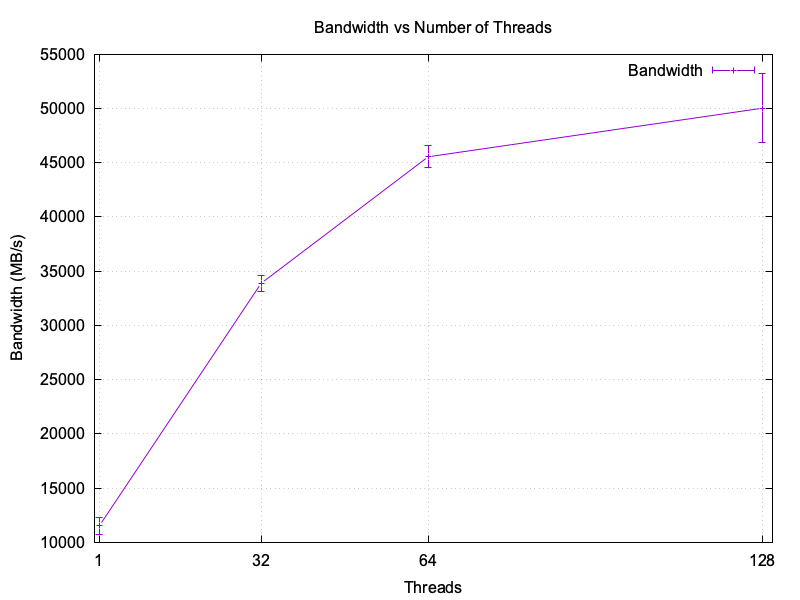
\includegraphics[width=0.9\textwidth]{img/ex2/ex2_threads.png}
  \caption{Stream bandwidth vs \#threads}
  \label{fig:ex2-threads}
\end{figure}

\subsection{Question 3: How does the measured bandwidth with the copy kernel depend on the number of threads?}
As depicted in \ref{fig:ex2-threads}, increasing the threads improves the bandwidth significantly.
The bandwidth is proportional to the number of threads, approachung a pleateu around 50GBit/s.

\subsection{Question 4: Prepare another plot comparing the bandwidth measured with copy kernel with static, dynamic, and guided schedules using 128 threads.}
\begin{figure}[H]
  \centering
  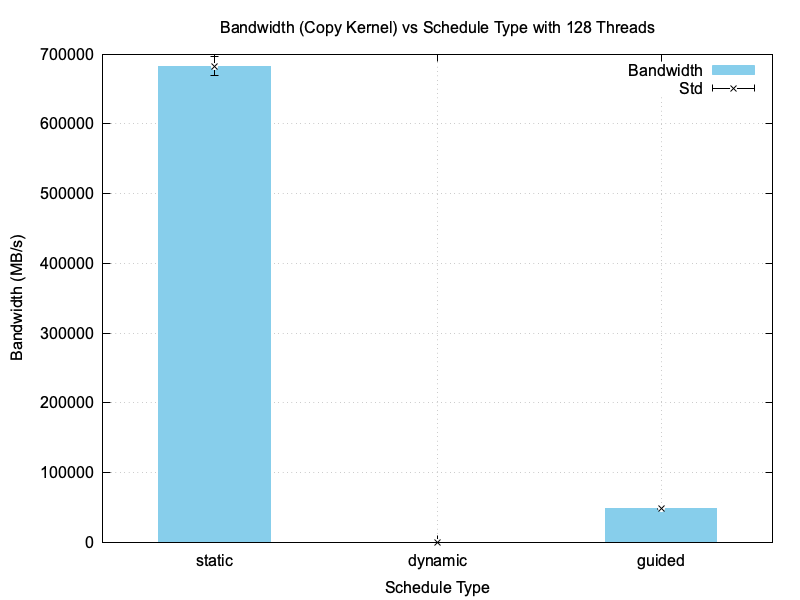
\includegraphics[width=0.9\textwidth]{img/ex2/ex2_schedule.png}
  \caption{Stream bandwidth for different schedulings}
  \label{fig:ex2-schedule}
\end{figure}
\subsection{Question 5: How do you set the schedule in the STREAM code? What is the fastest schedule, and why?}
To use different scheduler, we used the omp pragma \verb|omp parallel for schedule(runtime)| and set the environment variable using \verb|export OMP_SCHEDULE=<static,dynamic,guided>|.
We saw a huge difference in performance, to the point one might call it shocking.
By far the best performance was the static scheduling.
It outperformed the second best (guided sheduling) by magnitudes.
To me this looks suspecious, but double checking the scripts, everything else was the same.
The dynamic scheduler performed so bad, it's bar is not even really visible in the plot.
All this indicates to us, that the omp overhead is magnitudes more influencial than the runtime within the loop.

\section{Exercise 3 - Parallel Sum}
For this section, the job scripts that were used to run the experiments on Dardel can be found under the \verb|job_scripts/| directory \href{https://github.com/paulmyr/DD2356-MethodsHPC/tree/master/3_open_mp/exercise3/job_scripts}{here}. In general, we used 1 node and 128 logical CPUs on Dardel for all our experiments. 

The outputs generated and plotted from the scripts can be found \href{https://github.com/paulmyr/DD2356-MethodsHPC/tree/master/3_open_mp/exercise3/outputs}{here}. 

The code for the different implementations of the summation algorithm can be found \href{https://github.com/paulmyr/DD2356-MethodsHPC/tree/master/3_open_mp/exercise3}{here}.

To initialize, the arrays in each run, we used a seed of 42. The arrays had $10^8$ elements each. This helped us ensure the correctness of the results across different implementations. We repeated the experiment 10 times before reporting the average run for a given setting (given number of threads for the parallel implementations, for example). 

\subsection{Serial Performance}
The average time for the serial code was 0.332 seconds, with a standard deviation of 0.000995 seconds. This can be seen in \href{https://github.com/paulmyr/DD2356-MethodsHPC/blob/master/3_open_mp/exercise3/outputs/serial_output.txt}{this} output file.

\subsection{Implementing \textit{omp\_sum}}
The code for \verb|omp_sum| can be found in \href{https://github.com/paulmyr/DD2356-MethodsHPC/blob/master/3_open_mp/exercise3/omp_sum.c}{this} file. Here, we just add the \verb|#pragma omp parallel for| directive above the thread responsible for computing the sum. We used the allocation above -- 1 task per node with 128 CPUs per task. Using this and the job script \href{https://github.com/paulmyr/DD2356-MethodsHPC/blob/master/3_open_mp/exercise3/job_scripts/omp_sum_job.sh}{here}, we observed the following results (the speedup was computed by comparing with the serial runtime described above). 


\begin{table}[h!]
\centering
\begin{tabular}{|c|c|c|}
\hline
\textbf{Threads} & \textbf{Runtime w/ Std Dev (seconds)} & \textbf{Speedup} \\
\hline
1 Thread  & $0.325 \pm 0.000099$  & $1.021$ \\
2 Threads & $0.578 \pm 0.003681$  & $0.574$ \\
4 Threads & $0.505 \pm 0.002134$  & $0.657$ \\
8 Threads & $0.455 \pm 0.002015$  & $0.730$ \\
16 Threads & $0.423 \pm 0.001298$ & $0.785$ \\
20 Threads & $0.571 \pm 0.001688$ & $0.581$ \\
24 Threads & $0.635 \pm 0.002522$ & $0.523$ \\
28 Threads & $0.508 \pm 0.001187$ & $0.653$ \\
32 Threads & $0.876 \pm 0.000649$ & $0.378$ \\
64 Threads & $0.834 \pm 0.001449$ & $0.398$ \\
128 Threads & $0.745 \pm 0.007486$ & $0.446$ \\
\hline
\end{tabular}
\caption{Measurements for Simple \textit{omp\_sum} Implementation}
\end{table}

As can be seen with the outputs produced by the algorithm \href{https://github.com/paulmyr/DD2356-MethodsHPC/blob/master/3_open_mp/exercise3/outputs/omp_output.txt}{here}, apart from when we use 1 thread, the sum computed is incorrect when multiple threads are used. This is in line with our expectations. 

This is because of the lack of critical region protection for the piece of code that updates the \verb|sum_val| variable. Multiple threads can attempt to perform this update at the same time, and since this is not atomic, it can lead to inconsistent and different (and thus incorrect) results.  

As mentioned above, we allocated 128 logical CPUs for these runs for the different threads we experimented with. Thus, the \href{https://github.com/paulmyr/DD2356-MethodsHPC/blob/master/3_open_mp/img/ex3/ex3_topology_omp_sum.svg}{following} hierarchy infrastructure was allocated to us for performing the runs above. For all cases, apart from when 1 thread was used, the speed-up for all other runs was was less than 1, meaning it was even worse than sublinear. We believe that the reason for this poor performance could be the frequent updates to the same shared varible \verb|sum_val| by multiple threads at once. This would cause cache-invalidation, and thus not promote re-use of cache -- as each update to the shared \verb|sum_val| would force the thread to not be able to read the variable from cache. 

When only one thread was used, the speedup is close to 1 -- meaning the the runtime for this case was similar to the serial version. 

\subsection{Implementing \textit{omp\_critical\_sum}}
This implementation can be found \href{https://github.com/paulmyr/DD2356-MethodsHPC/blob/master/3_open_mp/exercise3/omp_critical_sum.c}{here}. The output (runtime, standard deviation, along with the sums) can be found in the file \href{https://github.com/paulmyr/DD2356-MethodsHPC/blob/master/3_open_mp/exercise3/outputs/omp_critical_output.txt}{here}. As can be seen by the outputs, no matter the number of threads used, the output is the same and above all, is correct (compared to the serial output). 

However, no matter how many threads we use, the runtime of this implementation is worse compared to the implementation of \verb|omp_sum| above and to the serial implementation. The \verb|critical| directive ensures that only 1 thread can execute the \verb|sum_val| update at a time. Thus, with the increase in the number of threads, contention to perform this update among the threads increases as well. So, with an increase in the number of threads, we see an increase in the runtime as well. Interestingly, even with just 1 thread, there is an increase in the runtime for the \verb|critical_sum| implementation. This indicates to us that there might be some overhead in establishing the critical section with the \verb|critical| directive, which would only add to the contention-related performance losses seen when even more threads are involved.

Plots comparing the runtimes of the different implementations along with the number of threads is available at the end of this section.

\subsection{Implementing \textit{omp\_local\_sum}}
The implementation can be found \href{https://github.com/paulmyr/DD2356-MethodsHPC/blob/master/3_open_mp/exercise3/omp_local_sum.c}{here}. The outputs produced for different thread counts (including standard deviation, the sum computed and the time taken) can be found \href{https://github.com/paulmyr/DD2356-MethodsHPC/blob/master/3_open_mp/exercise3/outputs/omp_local_output.txt}{here}. The output shows that in each run, no matter the number of threads, the same and the correct sum is computed. 

The performance of this implementation seems to be a lot better than the previous implementations. Its improved performance over the \verb|omp_critical_sum| implementation can be explained by the fact that we are not using any critical region in the computation of the sum. Thus, multiple threads can operate on their own copy of a local sum at the same time, which eliminates a bottleneck. 

It's already better than the \verb|omp_sum| implementation since it produces a correct output. Moreever, it also generally seems to be faster when using multiple threads (the performance with 1 thread is similar). We believe that this might be because of fewer cache-coherency/false-sharing issues with this implementation compared to the incorrect implementation of \verb|omp_parallel|. Here, each thread is responsible for computing the and storing its own \textit{local} sum in an index of the shared array. While there could still be some false-sharing between the array elements between the threads, the runtimes obtained here indicate that it is much better compared to the definitive false-sharing/cache-coherency issues cased by the \verb|omp_parallel| implementation. 

As above, a graph comparing the runtimes of the different implementations with varying threads are available at the end of this section.

\subsection{Implementing \textit{omp\_local\_sum} Without False-Sharing}
This implementation can be found \href{https://github.com/paulmyr/DD2356-MethodsHPC/blob/master/3_open_mp/exercise3/omp_local_no_sharing_sum.c}{here}. We create a new data structure to store the local-sums, where each element stores the local-sum for the individual thread, along with some padding. The cache-line size on dardel compute nodes was determined to be 64 bytes using the following command 

\begin{center}
\verb|srun getconf LEVEL1_DCACHE_LINESIZE|
\end{center}

Thus, we padded each local-sum with a 56 byte char array (with 8 bytes used by the local-sum of type \verb|double|).  With this, our hope is that each local-sum is on its own cache-line, which will help eliminate false-sharing between threads and solve cache-coherency, leading to (hopefully) better runtimes. 

The outputs produced with this implementation can be seen \href{https://github.com/paulmyr/DD2356-MethodsHPC/blob/master/3_open_mp/exercise3/outputs/omp_local_no_sharing_output.txt}{here}. Here, we also see that the output sum computed is the same for all threads (in all runs), and is correct. 

We see that this implementation seems to perform the best as the number of threads increase. This is in accordance with our expectations. 

Next, we present a graph which compares the runtimes for the different implementations as we change the number of threads.

\subsection{Final Plot of Runtimes}

\begin{figure}[H]
  \centering
  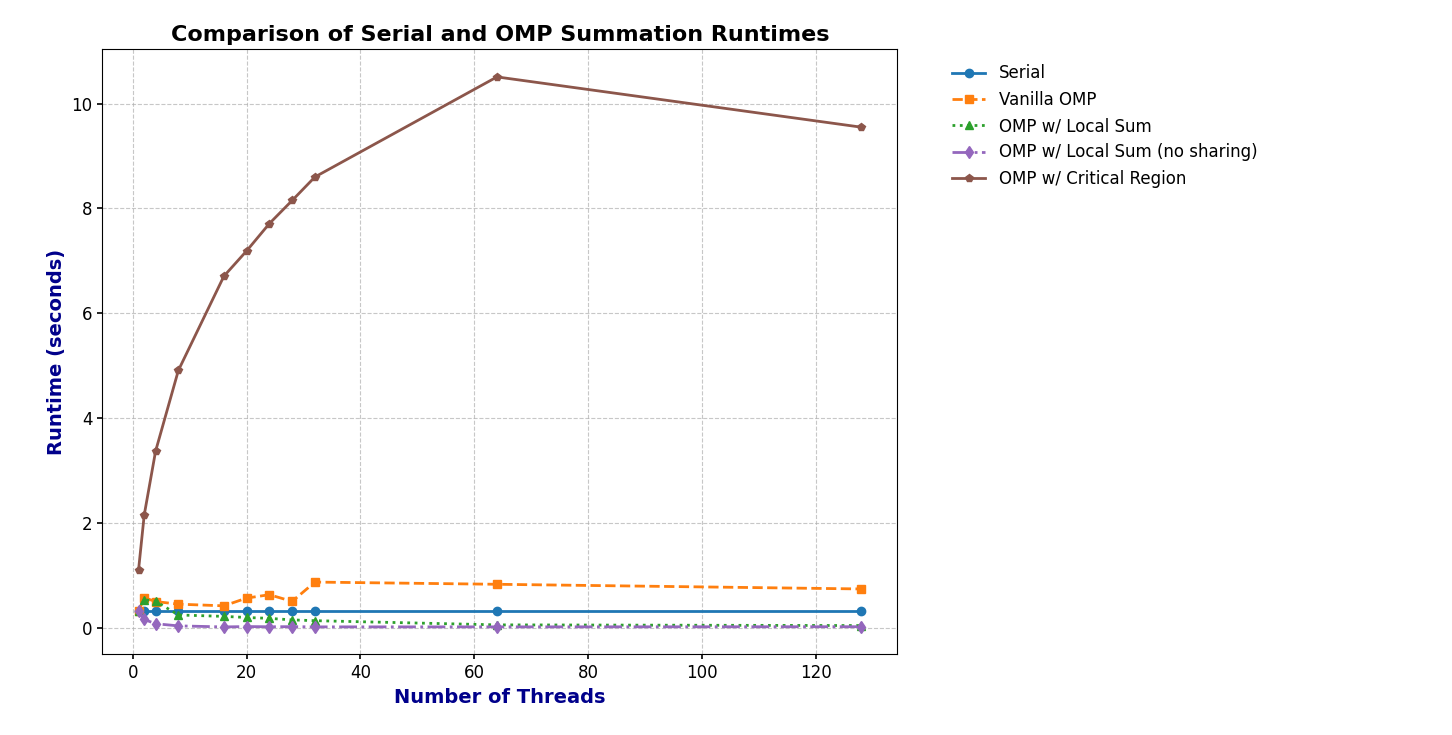
\includegraphics[width=0.9\textwidth]{img/ex3/ex3_comparison_all.png}
  \caption{Runtime Comparison of Different Implementations}
  \label{fig:ex3_runtime_all}
\end{figure}


The figure \ref{fig:ex3_runtime_all} shows the runtimes of the different implementations plotted against the number of threads. We can see that the OMP implementation with the critical region has the highest runtimes because of the reasons discussed above. The runtime is so large that it makes a visual comparison between the other implementations more difficult. 


\begin{figure}[H]
  \centering
  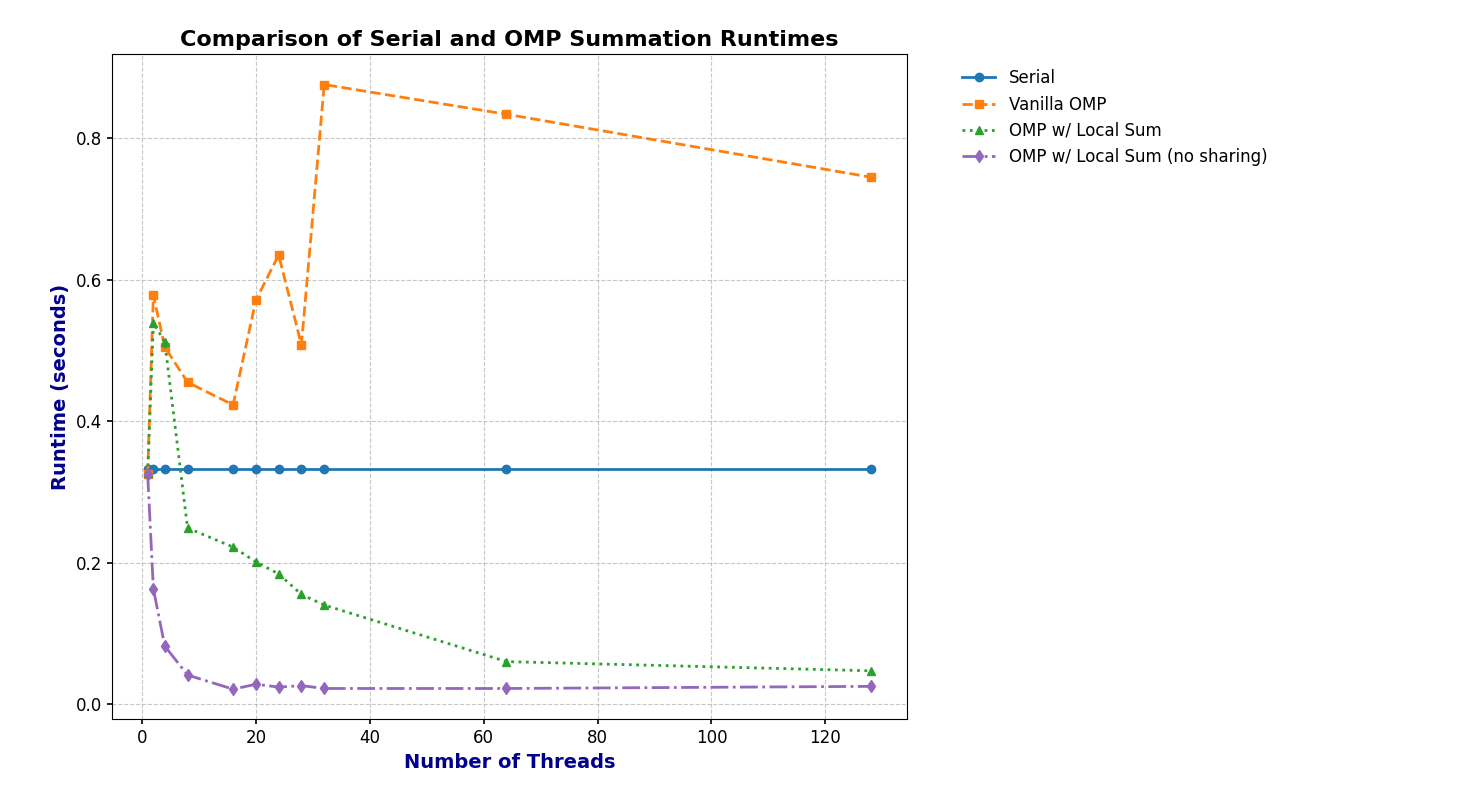
\includegraphics[width=0.9\textwidth]{img/ex3/ex3_comparison_no_critical.png}
  \caption{Runtime Comparison (without OMP w/ Critical)}
  \label{fig:ex3_runtime_no_critical}
\end{figure}

Figure \ref{fig:ex3_runtime_no_critical} shows the same runtimes without the outlier of \verb|OMP w/ Critical Region|. Here, we can see that the local sum implementation, where each thread computes its own local sum in parallel and then we serially combine the individual local sums, combined with padding to avoid false sharing of local sums between threads -- performs the best. The reasons for this has been analyzed earlier. 

\section{Exercise 4 - The Fastest DFT in the West}
The code for this section can be found under the \verb|excersie4/| directory in the project repository (\href{https://github.com/paulmyr/DD2356-MethodsHPC/tree/master/3_open_mp/exercise4}{here}). 

\subsection{A Parallel Imlementation}
We went with a simple parallelization of the main \verb|for| loop responsible for the computation. We added a \verb|#pragma omp parallel for| directive above the outer for-loop. This divided the responsibility of computing the different indices of the \verb|Xr_o| and \verb|Xi_o| arrays to different threads in the parallel implementation. The relevant code directive was added at \href{https://github.com/paulmyr/DD2356-MethodsHPC/blob/master/3_open_mp/exercise4/dftw_parallel.c#L88}{this} line to the original code. The file with the parallel code is \verb|dftw_parallel.c|, which can be found \href{https://github.com/paulmyr/DD2356-MethodsHPC/blob/master/3_open_mp/exercise4/dftw_parallel.c}{here}.


\subsection{Performance Measurement}
We assumed that 32 cores here meant \underline{physical cores}. Thus, all performance measurements were made requesting 64 \underline{logical cores} on dardel. Using an input size of $N = 10000$, we get a serial runtime average of 17.5188071 seconds and a standard deviation of about 0.002749 seconds. Compared to the serial implementation, Table \ref{table:ex4_64_cores} summarizes the average runtime and standard deviation for the parallel implementation (using the strategy above). \href{https://github.com/paulmyr/DD2356-MethodsHPC/blob/master/3_open_mp/exercise4/job_scripts/dftw_parallel_job.sh}{This} was the job script for the 64 logical cores run.

\begin{table}[h!]
\centering
\begin{tabular}{|c|c|c|}
\hline
\textbf{Threads} & \textbf{Runtime w/ Std Dev (seconds)} & \textbf{Speedup} \\
\hline
1 Thread  & $17.5795922 \pm 0.005705$  & $0.99654229$ \\
32 Threads & $0.5625909 \pm 0.003324$ & $31.13951381$ \\
64 Threads & $0.4102998 \pm 0.006772$ & $42.6975765$ \\
128 Threads & $0.4916456 \pm 0.023272$ & $35.63299885$ \\
\hline
\end{tabular}
\caption{Measurements for Parallel DFTW on 32 Physical (64 Logical) Cores}
\label{table:ex4_64_cores}
\end{table}

We notice an increase in runtime (and decrease in speed-up) in going from 64 to 128 threads. This is likely because of the fact that there are fewer (logical) cores available than there are threads, and thus there is contention and scheduling overhead which hinders the amount of work which can be done by the 128 threads. This is confirmed by the fact that when we run the program on 128 logical cores, the runtime using 128 threads is the fastest (\href{https://github.com/paulmyr/DD2356-MethodsHPC/blob/master/3_open_mp/exercise4/job_scripts/dftw_parallel_all_cores_job.sh}{this} was the job-script for the 128-core run), as seen in Table \ref{table:ex4_128_cores}. 

\begin{table}[h!]
\centering
\begin{tabular}{|c|c|c|}
\hline
\textbf{Threads} & \textbf{Runtime w/ Std Dev (seconds)} & \textbf{Speedup} \\
\hline
1 Thread  & $17.5752934 \pm 0.004707$  & $0.99678604$ \\
32 Threads & $0.5612639 \pm 0.000900$ & $31.21313717$ \\
64 Threads & $0.3177174 \pm 0.002636$ & $55.13958977$ \\
128 Threads & $0.2221419 \pm 0.011786$ & $78.86313703$ \\
\hline
\end{tabular}
\caption{Measurements for Parallel DFTW on 64 Physical (128 Logical) Cores}
\label{table:ex4_128_cores}
\end{table}

The files containing the outputs for the 2 runs above can be found \href{https://github.com/paulmyr/DD2356-MethodsHPC/blob/master/3_open_mp/exercise4/outputs/dftw_omp_output_64.txt}{here} (for the 64 logical cores) and \href{https://github.com/paulmyr/DD2356-MethodsHPC/blob/master/3_open_mp/exercise4/outputs/dftw_omp_output_128.txt}{here} (for the 128 logical cores). They also illustrate that the parallel code remains correct (with the output of the \verb|checkResults| function in the original code). There was a script which parsed these files and produced a summary of results and the plots (in the next section), which can be found \href{https://github.com/paulmyr/DD2356-MethodsHPC/blob/master/3_open_mp/exercise4/outputs/plotting_script_output.txt}{here}. The script itself can be found \href{https://github.com/paulmyr/DD2356-MethodsHPC/blob/master/3_open_mp/exercise4/parse_output_and_plot.py}{here}.

\subsection{Performance and Speed-Up Plot}

Figure \ref{fig:ex4_performance} shows the raw performance comparison as a function of number of threads for the serial implementation compared to the parallel ones on different number of logical cores. These values are plotted from the tables above, and show the pattern discussed there.

\begin{figure}[H]
  \centering
  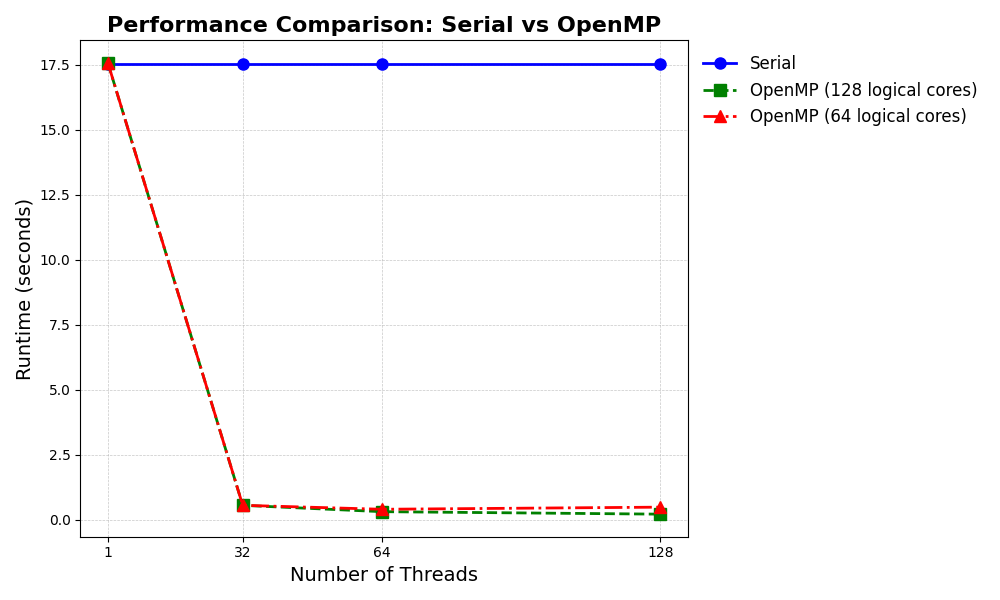
\includegraphics[width=0.9\textwidth]{img/ex4/performance_comparison.png}
  \caption{Runtime Comparison of Parallel and Serial}
  \label{fig:ex4_performance}
\end{figure}

Figure \ref{fig:ex4_speedup} shows the speedup of the parallel implementation on different number of logical cores. As argued earlier, the speeup keeps getting better (although with a lower rate of improvement) as the number of threads increase for 128 (logical) cores compared to 64 (logical) cores. The reason for this was discussed earlier.
\begin{figure}[H]
  \centering
  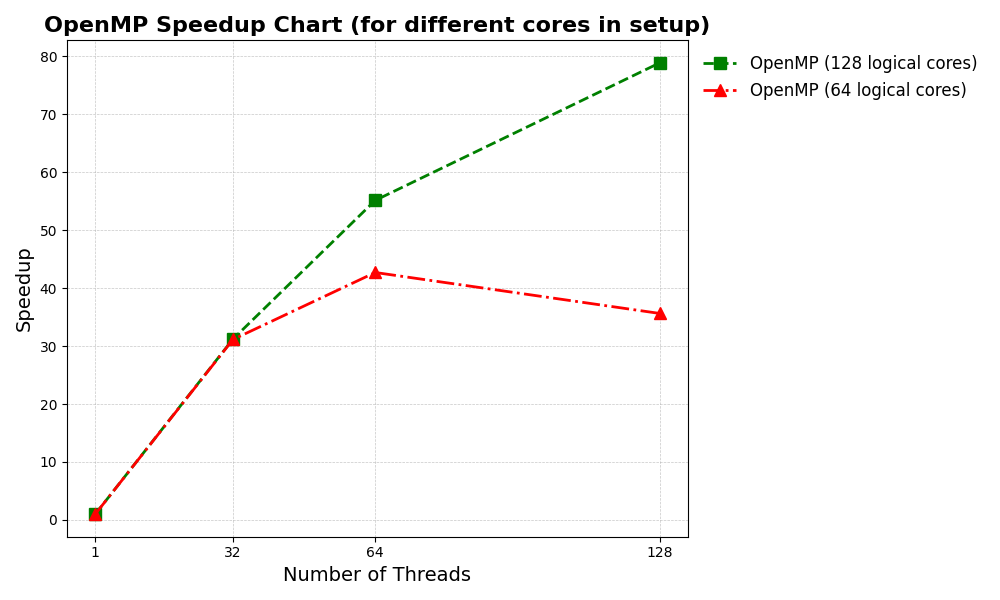
\includegraphics[width=0.9\textwidth]{img/ex4/speedup_plot.png}
  \caption{Speedup Plot}
  \label{fig:ex4_speedup}
\end{figure}



\subsection{Non-Parallel Performance Optimizations}
\todo{Not entirely sure what to write here...maybe loop order change to prevent cache misses?}

\section{Exercise 5 - Parallelizing a Shallow Water Simulation}
\subsection{1. Parallelize the loops}
We parallelize the loops given the \verb|#pragma omp parallel for collapse(2)| pragma. 
We implement the different scheduling strategies in the slurm file with is attached to the repository (ex5.slurm).
The timing of the \verb|compute()| method is measured using \verb|omp_get_wtime()|.
The code is run on the cluster using a jobarray in the slurmfile, where we iterate through the permuations.

\subsection{2. Evaluate Performance}
All the data can be found in the repo (\href{https://github.com/paulmyr/DD2356-MethodsHPC/tree/master/3_open_mp/exercise5/data}{Dataset directory}).
We evaluate based on scheduling strategy, gridsize ($N$) and threadcount ($threads$).

For our static scheduling, we observe the fastest exectution for a chunksize of $ 1000 $ for $64 threads$ and a gridsize $N=500$ with $0.040567 s$.
The results (present in the file \verb|df_static.csv|) display the six fastest calculations for $64 threads$ and $N=500$, which are surprisingly faster than a higher threadcount for the same gridsize.

For the dynamic scheduling, we assume even better results since the computational load could theoretically be better distributed. 
We observe the fastest exectution for a chunksize of $ 200 $ for $64 threads$ and a gridsize $N=500$ with $0.041169 s$.
The results (\verb|df_dynamic.csv|) display the four fastest calculations for $64 threads$ and $N=500$, which are interestingly again faster than a higher threadcount for the same gridsize.
Interestingly the dynamic scheduling is slower than the static scheduling.

For the guided scheduling (\verb|df_guided.csv|), we observe the following results. The fastest exectution time ($0.040684 s$) is archieved for $64 threads$ and a gridsize $N=500$ for a chunksize of $100$.
Again the $64 threads$ are superior to other thread counts.

We compare the gridsizes and threads for static scheduling with a chunksize of $1000$ and a threads being used kept to a constant of 64. When looking at different gridsizes we observe the results in Table \ref{table:ex5_grid_changes}:

\begin{table}[h!]
\centering
\begin{tabular}{|c|c|}
\hline
\textbf{Grid Size} & \textbf{Time} \\
\hline
500  & $0.040567$  \\
1000 & $0.124492$ \\
2000 & $0.445595$ \\
4000 & $3.1712616$ \\
8000 & $14.403611$ \\
\hline
\end{tabular}
\caption{Runtimes for Different Grid Sizes (1000 chunk size, 64 threads, static schedule)}
\label{table:ex5_grid_changes}
\end{table}

Unsurprisingly with a larger gridsize the runtime increases for constant parameters.


When looking at different thread counts we observe the data in Table \ref{table:ex5_thread_changes}. We keep a constant grid size of 500 and a static schedule with a chunk size of 1000 (for reference, the serial runtime for a grid size of 500 was found to be 1.387342 seconds):
\begin{table}[h!]
\centering
\begin{tabular}{|c|c|c|}
\hline
\textbf{Threads} & \textbf{Runtime} & \textbf{Speedup} \\
\hline
1 Thread  & $1.45063$  & $0.95637$ \\
32 Threads & $0.051778$ & $26.7940$ \\
64 Threads & $0.040567$ & $34.19878$ \\
128 Threads & $0.067249$ & $20.62993$ \\
\hline
\end{tabular}
\caption{Runtimes for Different Thread Counts (1000 chunk size, static schedule, 500 grid size)}
\label{table:ex5_thread_changes}
\end{table}

Interestingly after 64 threads, the speedup decreases again, which we assume to be due to overhead of creating and managing a higher number of thread (such as scheduling, spawning, etc).

\subsection{3. Visualize the output}
The figure below shows the output for a gridsize of $N=500$ calculated using $32 threads$ and the \verb|OMP_SCHEDULE| set to dynamic with a 
chunksize of $ 100 $.
The exectution time of the parallel exectution takes $0.052771s$ while the serial computation for the same gridsize of $N=500$ takes $1.387342s$.  
This leaves us with a \verb|speedup ratio| ($speedup = Time_serial / Time_parallel$) of $speedup = 1.387342s/0.052771s = 26.28986 $. 


\begin{figure}[H]
  \centering
  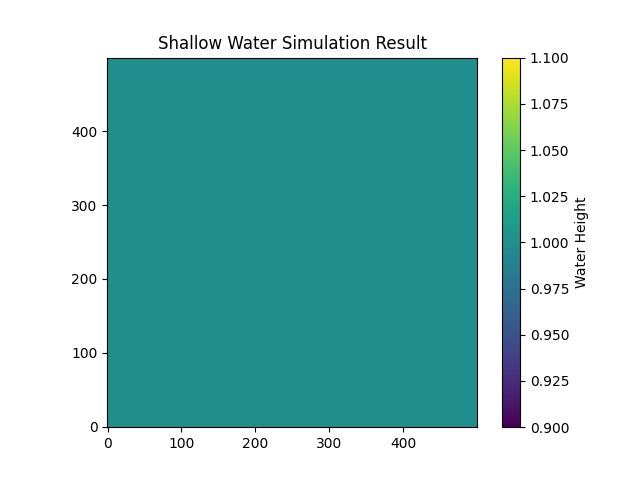
\includegraphics[width=0.9\textwidth]{img/ex5/parallel_plot.png}
  \caption{Parallel Plot}
  \label{fig:ex5_parallel}
\end{figure}

To check the correctness of our results, we plot the serial implementation result below which displays the same water simulation result.

\begin{figure}[H]
  \centering
  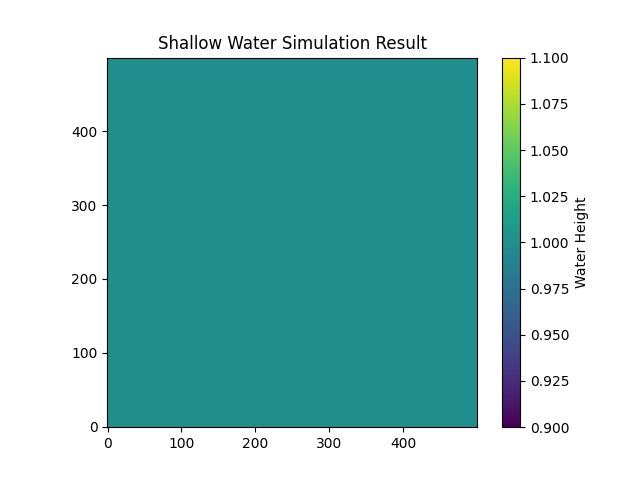
\includegraphics[width=0.9\textwidth]{img/ex5/serial_plot.png}
  \caption{Parallel Plot}
  \label{fig:ex5_serial}
\end{figure}


The code and slurmfile to replicate our results are attached to the repository.

\section{Bonus -- Simulating Neurons with OpenMP Tasks}
\textit{Note: The GPU bonus is not included here, as dardel was not able to support the requirements of the task, as stated in the announcement.}

All the results in this section were obtained after running the programmes on 64 physical cores (ie, 128 logical cores) on dardel. The job-scripts that were used to run the programmes can be found \href{https://github.com/paulmyr/DD2356-MethodsHPC/tree/master/3_open_mp/bonus/neuron/job_scripts}{here}, and the program implementation themselves can be found in the files \verb|neural_serial.c| (\href{https://github.com/paulmyr/DD2356-MethodsHPC/blob/master/3_open_mp/bonus/neuron/neuron_serial.c}{here}) and \verb|neuron_omp.c| (\href{https://github.com/paulmyr/DD2356-MethodsHPC/blob/master/3_open_mp/bonus/neuron/neuron_omp.c}{here}). 

Note that to ensure that we can verify correctness of the parallel implementation with the serial implementation, we have altered how the random numbers are generated in determining the triggering of neurons. Instead of using the \verb|rand()| function, we pre-generate the seeds outside the parallel region, and then read the seeds from this array for the correct \verb|(neuron, step)| combination. This can be seen in the modified code for the \verb|compute()| method in both the implementations. 

\subsection{Implementation and Correctness}
The OMP task implementation can be found in the file \verb|neuron_omp.c| \href{https://github.com/paulmyr/DD2356-MethodsHPC/blob/master/3_open_mp/bonus/neuron/neuron_omp.c}{here}. We have followed the steps highlighted in the handout, and that were illustrated in \href{https://stackoverflow.com/questions/68502197/how-do-omp-single-and-omp-task-provide-parallelism}{this} resource explaning how \verb|omp task| works with \verb|omp single|, since this was not covered in the course materials. 

To verify the correctness, we examined the diff of the summary output generated by the serial implementation and the summary generated by the parallel implementation for differing number of threads (keeping the other parameters constant). These are present in the \verb|threads_summary/| directory \href{https://github.com/paulmyr/DD2356-MethodsHPC/tree/master/3_open_mp/bonus/neuron/threads_summary}{here}. The outputs of the \verb|*_threads_<number>.txt| files is the same as the output of the \verb|*_threads_serial.txt| file.

% The correctness can also be verified for the different runs where we varied the neuron counts and the threshold, keeping the number of threads at a constant of 64. For the varying neuron counts, the summaries are present in the \verb|counts_summary/| directory (\href{https://github.com/paulmyr/DD2356-MethodsHPC/tree/master/3_open_mp/bonus/neuron/counts_summary}{here}). We can compare the \verb|*_count_serial_<number>.txt| summary with the \verb|*_count_<number>.txt| summary and see they're the same.
\subsection{Performance Comparison (Varying Threads)}
\begin{figure}[H]
  \centering
  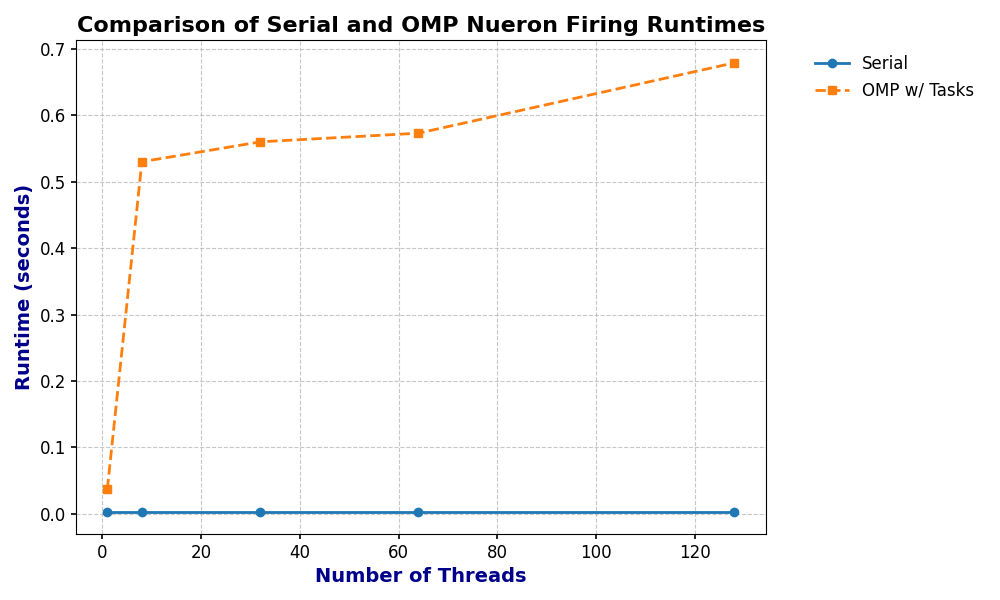
\includegraphics[width=0.9\textwidth]{img/bonus/performance_thread_variation.png}
  \caption{Serial vs OMP Task Neuron Simulation}
  \label{fig:bonus_performance}
\end{figure}

Figure \ref{fig:bonus_performance} shows the runtime changes as a function of threads for the serial implementation and the OMP tasks implementation. The data used to generate this plot can be found in the \verb|outputs/| directory (\href{https://github.com/paulmyr/DD2356-MethodsHPC/blob/master/3_open_mp/bonus/neuron/outputs/neuron_omp_job.results}{here}). 

As the figure shows, the implementation with OMP tasks is a lot slower compared to the serial implementation. This is despite the use techniques such as padding to remove false sharing on top of OMP parallelization. To us, this illustrates the drawback of using OMP tasks for this workload. 

Task based parallelism is said to be the prefferred approach when there is irregular workloads to be dealt with in parallel. However, the indpendent update of each neuron here seems to be a consistent amount of work (if we assume that the conditional update of the potential if it reaches beyond the threshold is a negligible amount of work).

 Thus, it is likely the case that the overhead of using task-based parallelism as the approach here -- of spawning threads, delegating the work of creating tasks to a single thread, executing the tasks, etc -- hinders any advantage offered by parallelism, and the figure \ref{fig:bonus_performance} supports our hypothesis. 

\subsection{Task vs Loop Parallelism}
Task Parallelism with OMP is a preferred approach when there is independent work to be done at the same time -- where each unit of work could take a varying amount of time. This involves spawning threads using the \verb|omp parallel| directive, distributing tasks to these threads (can be done by a single thread using the \verb|omp single| directive), and then the spanwed threads executing the independent tasks in the \verb|omp task| region distributed earlier. 

On the other hand, Loop Parallelism is a specific type of parallelism, where the individual iterations of a loop are parallelized using the \verb|omp for| directive. Here, individual iterations of the loop are distributed amongst the threads spawned in the \verb|omp parallel| region. This distribution and execution of the loop iterations can be done on a specific schedule. Generally, each iteration of the loop would take around the same amount of work to finish, and would be independent to gain full advantage of parallelism.

\subsection{Neural Connections as Task Dependencies}
In this simulation, we have a random signal that alters the potential of each neuron and determines whether the neuron has been fired or not. However, we can make the model more complex by altering the potential of a neuron based on the potential of other (neighbouring) neurons. This would simulate a connection between neurons, as the potential of one neuron (ie, its \textit{output}) would depend on the potential of neighbouring neurons (ie, their \textit{input} provided to the neuron). 

This can be implemented using OMP tasks with the \verb|omp task depend| directive. We can then specify the \textit{input} and \textit{output} potential requried and produced (respectively) by each neuron with the help of the \verb|omp task depend (in:...)| and \verb|omp task depend (out:...)| commands.   

\subsection{Performance Comparison (Varying Nuerons)}
\begin{figure}[H]
  \centering
  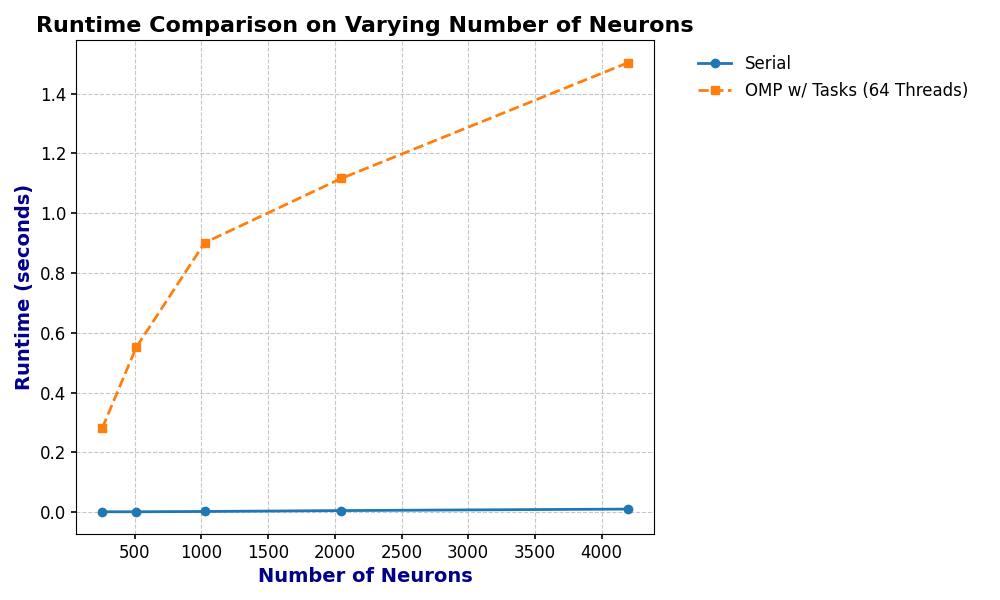
\includegraphics[width=0.9\textwidth]{img/bonus/neuron_variation.png}
  \caption{Serial vs OMP Task (64 Threads) Varying Neuron Count}
  \label{fig:bonus_neuron}
\end{figure}

We compared the OMP task and the serial implementation by varying the number of neurons and keeping the other elements constant. The output produced can be found in the \verb|neuron_omp_count_job.results| file (\href{https://github.com/paulmyr/DD2356-MethodsHPC/blob/master/3_open_mp/bonus/neuron/outputs/neuron_omp_count_job.results}{here}). We kept the number of threads at a constant 64 for the OMP task implementation. The results are present in the plot in Figure \ref{fig:bonus_neuron}. We clearly see that an increase in the number of neurons leads to an increase in the runtime (if we keep the number of threads constant). This slight increase is seen in the serial runtime as well, but to a much lesser extent.

The increase in runtime with the OMP Task implementation can be explained with the fact that there are more independent neuron updates to do with an increase in the number of neurons, and thus more scheduling and OMP task related overhead to manage as well. Thus, the slower performance with fewer number of neurons is exaggerated as the number of neurons increase, resulting in the trend observed. 

In all cases though, the runtime of the OMP task implementation is much more than the serial implementation, and we have discussed the likely causes of this earlier. 

\subsection{Neuron Activity and Firing Threshold}
While the runtime comparison was not asked for this task in the handout, a textual runtime comparison of the serial implementation and the OMP Task implementation (with 64 threads) is available in the \verb|neuron_omp_threshold_job.results| file (\href{https://github.com/paulmyr/DD2356-MethodsHPC/blob/master/3_open_mp/bonus/neuron/outputs/neuron_omp_threshold_job.results}{here}). We vary the threshold and keep the other factors (threads, neuron counts, etc) constant. 

Varying the threshold would only have change the number of times the conditional potential reset for the neuron is executed, and thus for all threshold counts, we see very similar runtimes when the OMP Task runtimes are compared with each other as the threshold changes (same goes for the trend with the serial implementation). This re-inforces our conjecture that the amount of time spent in the \verb|if-| branch in the potential update of each independent task was negligible, and thus that each task was roughly the same amount of work (which would make OMP Task not ideal for this type of workload, as can be seen in the diminished runtime over serial). 

As the firing threshold increases, we would expect to see an increase in the neuron firing rate, as now lower bounds need to be crossed to trigger a neuron firing. Thus, for each neuron, we would expect higher firing times in the final summary. This is the trend seen if we plot the neuron firing-rate histogram using one of the plotting scripts provided. We visualize some of the histograms (for threshold 20, 200, and 500) in Figure \ref{fig:bonus_threshold}. The other plots can be seen in the \verb|img/bonus/| directory of the repository \href{https://github.com/paulmyr/DD2356-MethodsHPC/tree/master/3_open_mp/img/bonus}{here}.


\begin{figure}
\centering
\begin{subfigure}{0.4\textwidth}
    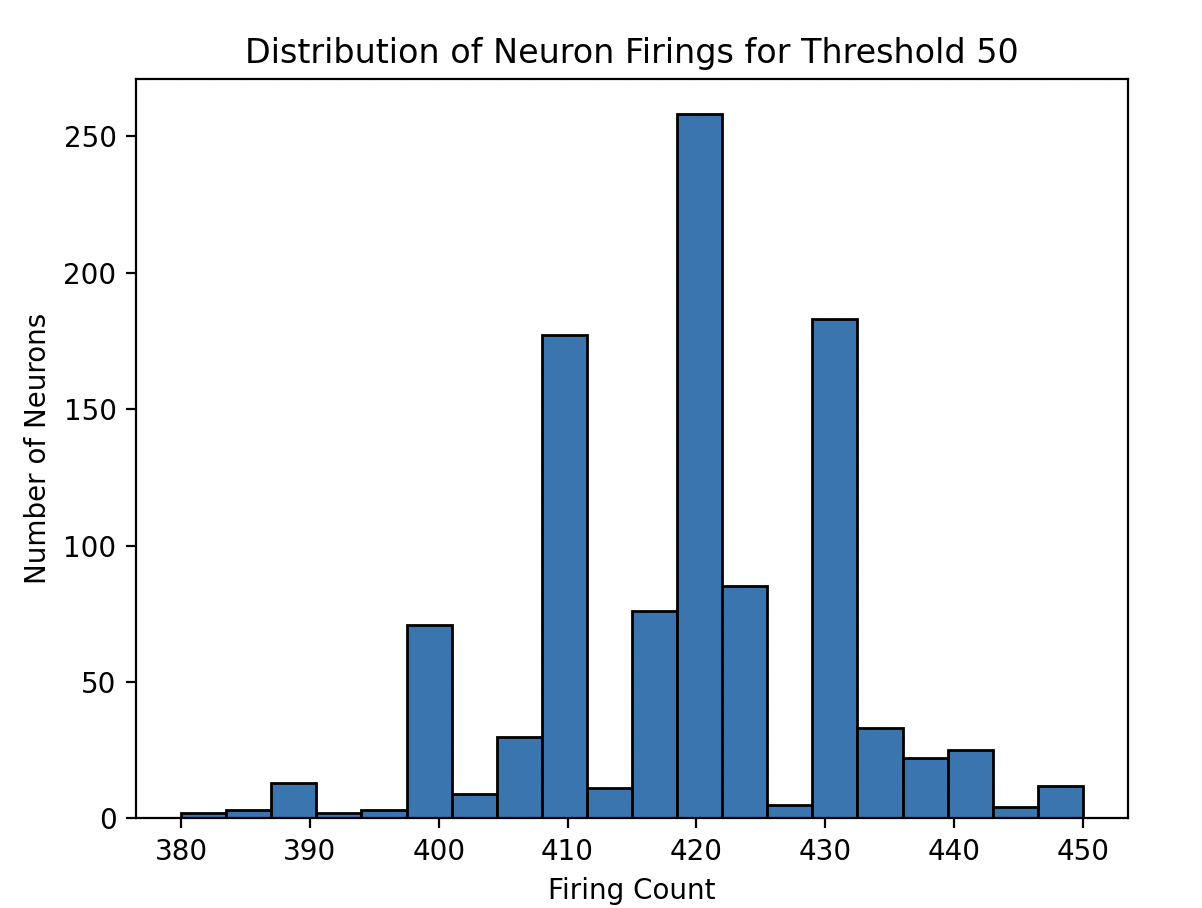
\includegraphics[width=\textwidth]{img/bonus/threshold_50.png}
    \caption{Threshold 20}
\end{subfigure}
\hfill
\begin{subfigure}{0.4\textwidth}
    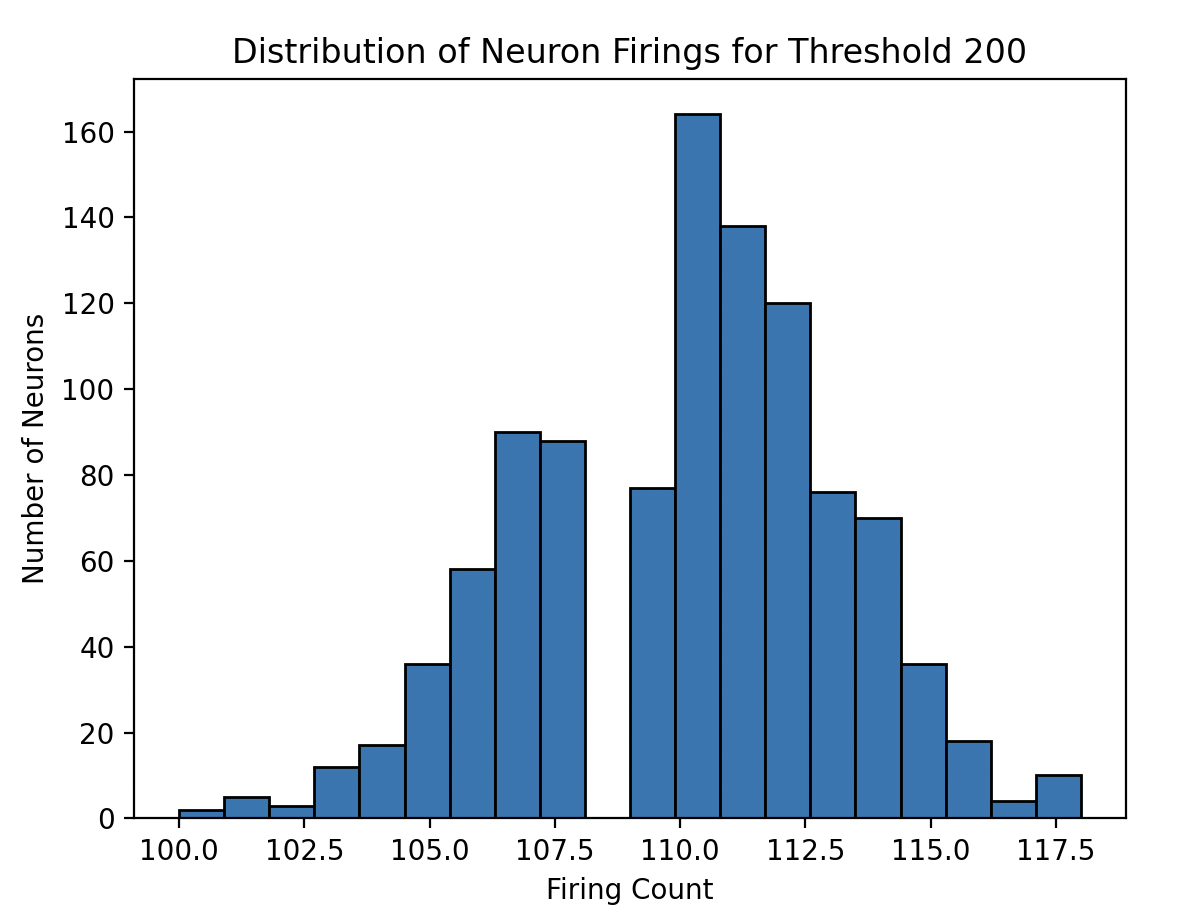
\includegraphics[width=\textwidth]{img/bonus/threshold_200.png}
    \caption{Threshold 200}
\end{subfigure}
\hfill
\begin{subfigure}{0.4\textwidth}
    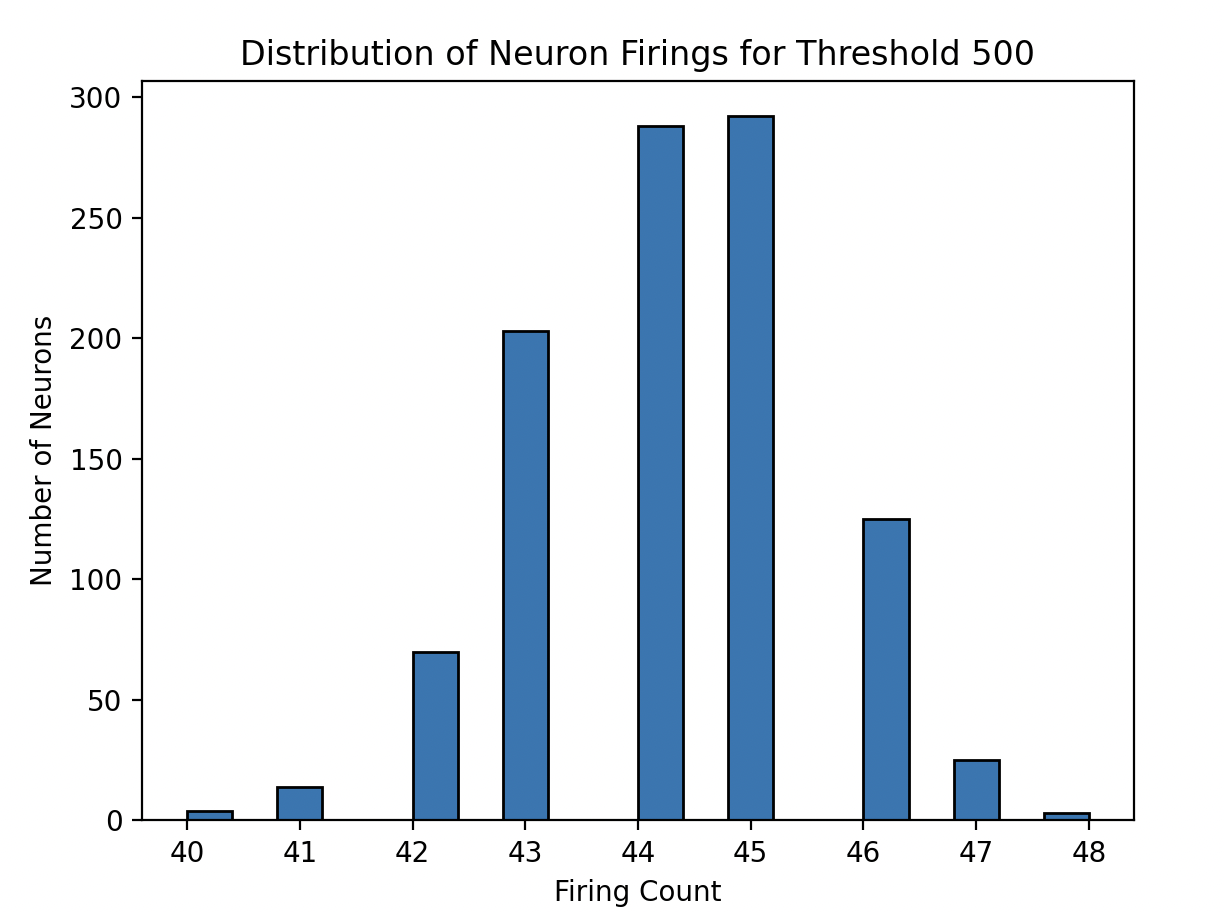
\includegraphics[width=\textwidth]{img/bonus/threshold_500.png}
    \caption{Threshold 500}
\end{subfigure}
\hfill
        
\caption{Neuron Firing Rates For Different Thresholds}
\label{fig:bonus_threshold}
\end{figure}

% content end
%###############################################################################

% \printbibliography

\end{document}
